\documentclass[12pt, block=fill]{beamer}
\usepackage[sfdefault]{FiraSans}
\usepackage{FiraMono}
\usepackage[T1]{fontenc}
\usepackage{xcolor}

\usepackage{pgfpages}
% \setbeameroption{hide notes} % Only slides
% \setbeameroption{show only notes} % Only notes
  \setbeameroption{show notes on second screen=right} % Both

\definecolor{burntOrange}{rgb}{.8, .5, .1}
\definecolor{textgray}{rgb}{.8,.8,.8}

\usetheme[titleformat frame = smallcaps]{metropolis}

\metroset{block=fill}

\newcommand{\E}{\text{E}}
\newcommand{\V}{\text{V}}
\newcommand{\cov}{\text{cov}}

\title{Hypothesis Testing} 
\subtitle{UC Berkeley, MIDS w203} 
\author{Statistics for Data Science}

\begin{document}

\maketitle

\section{Introducing the Two-Sample t-Test}

\begin{frame}
  \frametitle{Motivating the Two-Sample t-Test}
  \begin{exampleblock}{Comparing Two Metric Variables}
    Is group A different from group B in expectation?
  \end{exampleblock}

\note[item]{The two-sample t-test is one of the most common procedures in inferential statistics. What is it for? As a data scientist you will often face a question about two groups - group A and group B. Someone will ask you if one is greater or less than than the other.}
\note[item]{Questions like this are everywhere. In business, you have A-B testing.}
\note[item]{In medicine, you may want to test a group of patients taking a vitamin against a control group}
\note[item]{In political science, you may want to test whether democracies or autocracies start more wars.}
\note[item]{What do these questions have in common? They all have two groups, and in all cases we're measuring the outcome on a metric scale. So it makes sense to ask about the expectation of each population - are the expectations different?}


  Examples:
  \begin{itemize}
      \item Are customers who get a birthday gift less likely to leave than those who don't?
      \item Do patients who take Vitamin W get over the flu faster than patients who don't?
      \item Do democracies or autocracies start more wars?
  \end{itemize}
  \end{frame}

\begin{frame}
  \frametitle{Example Scenario}
  \note[item]{Here's a specific example, with data.}
  \note[item]{write on slide: 13.3-12.1 = 1.2 outfits}
  \note[item]{Is this a big difference? is it just noise?}
  \note[item]{To be more precise, is this evidence that SF'ans have more black outfits than NYers in general?}
  \note[item]{To analyze this question, we need a model...}
  \begin{exampleblock}{From the Journal of Empirical Fashion}
  \begin{tabular}{c | c | c}
  & New Yorkers & San Franciscans \\
  \hline
black outfits &  12.1 & 13.3  \\
sample size & 50 & 50
 \end{tabular}
 \end{exampleblock}
 
\vspace{1.5cm}
 Is this evidence that San Franciscans have more black outfits than New Yorkers \textit{in general}? \end{frame}
 
 
 \begin{frame}
  \frametitle{Two-Sample Model Framework}
  \note[item]{A model is a representation of the world built of RVs. for a two-sample t-test, the model begins like this.}
  \note[item]{Let $X_1.. X_{n_1}$ be RVs representing group A. Similarly for Y.}
  \note[item]{Let's assume that the X's are iid with mean $\mu_X$. same for Y}
  \note[item]{We'll need more assumptions, but this is a start.}
  \note[item]{The null is that our two means are the same.}
  \note[item]{Our usual alternative is that the means are different.}
  \note[item]{It is also possible to run a one-sided test in special circumstances. alt is one mean is greater than other.}
  \note[item]{Given this model, how plausible is the null hypothesis?}

  \begin{exampleblock}{Basic Model Setup} 
    Suppose $(X_1,..,X_{n_1})$ are i.i.d. with mean $\mu_X$.    
    
    Suppose $(Y_1,..,Y_{n_2})$ are i.i.d. with mean $\mu_Y$. 
       \end{exampleblock}

  \begin{exampleblock}{Null Hypothesis}
    $H_{0}: \mu_{X} = \mu_{Y}$ (The two groups' means are equal)
  \end{exampleblock}
  
  \begin{exampleblock}{Alternative hypotheses}
    $H_{1}: \mu_{X} \neq \mu_{Y}$ (best choice in most cases)\\
    $H_{2}: \mu_{X} > \mu_{Y}$ \\
    $H_{3}: \mu_{X} < \mu_{Y}$ 
  \end{exampleblock}
\end{frame}


\begin{frame}
  \frametitle{Comparing Population Means}
  \note[item]{One important piece of information is how much does the number of black outfits vary in the population.}
  \note[item]{Here's a picture with three different distributions for our sample averages.}
  \note[item]{The top distribution has very high standard deviation. You can see that it doesn't seem unusual to get two sample averages that are 1.2 outfits apart.}
  \note[item]{The middle distribution has medium deviation. Now it starts to look a little more surprising that our two sample averages were 1.2 apart.}
  \note[item]{The bottom distribution has low standard deviation. Now it seems quite unlikely to get two sample averages 1.2 apart. The data seems inconsistent with this hypothesis.}
    \begin{center}
        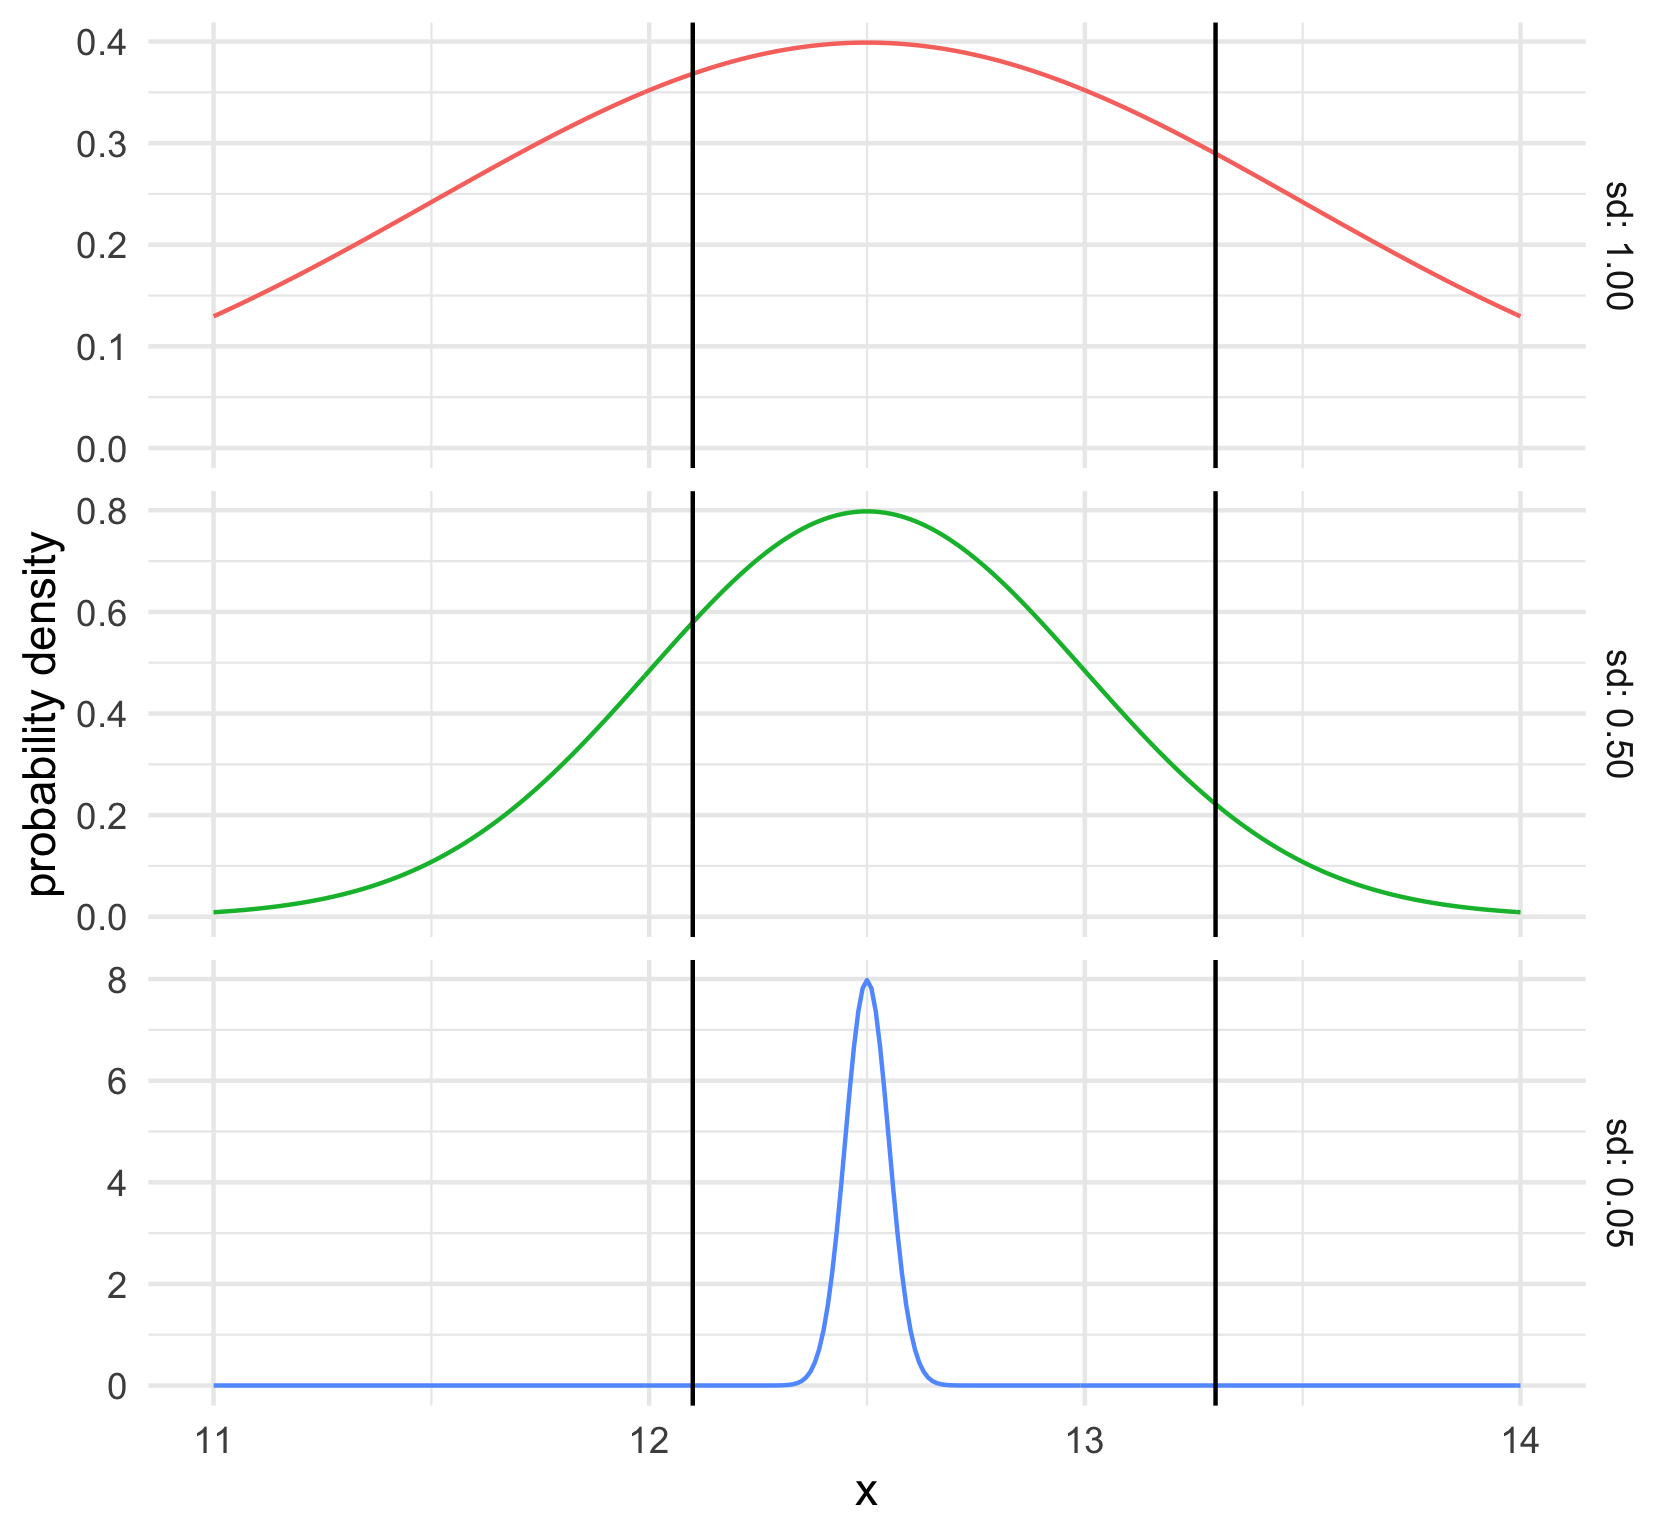
\includegraphics[width = 0.9\linewidth]{figures/fashion_plot.png}
    \end{center}
\end{frame}

\begin{frame}
  \frametitle{Comparing Population Means}
  \note[item]{Putting these ideas together, we can make a statistic by taking the difference in sample averages, and dividing by an estimate of standard deviation - that's exactly the idea behind the two- sample t-test}
  \begin{exampleblock}{Two-Sample t-Test}
  
 $$t = \frac{\bar X - \bar Y}{\text{Estimate of Standard Deviation}}$$
 
    Assess whether two populations have the same expectation \textbf{while accounting for variability}
  \end{exampleblock}


\end{frame}


%Section 7.06 Edits end


%Section 7.08 Edits start

\section{The Two-Sample z-Test}





\begin{frame}[t]
  \frametitle{Two-Sample \textit{z}-Test}
  \begin{exampleblock}{Assumptions} 
    Suppose $(X_1,..,X_{n_1})$ are i.i.d. with mean $\mu_X$.    
    
    Suppose $(Y_1,..,Y_{n_2})$ are i.i.d. with mean $\mu_Y$. 
    
    Assume $X \sim N(\mu_X, \sigma)$.  $Y \sim N(\mu_Y, \sigma)$.  We know $\sigma$.
      \end{exampleblock}
      \note[item]{Before we tackle the two-sample t-test, let's begin with the simpler 2 samp. z test. unrealistic, but build intuition.}
      \note[item]{Same assumptions as before, but add assump. of equal var $\sigma$ which we know.}
      \note[item]{How do we create a test statistic?}
      \note[item]{What is the distribution of $\bar{X} - \bar{Y}$? Let's use fact that a difference of normal RVs is normal. but which normal?}
      \note[item]{$V[\bar{X} - \bar{Y}] = V[\bar{X}] + V[\bar{Y}] = \sigma^2/n_1 +  \sigma^2/n_2$}
      \note[item]{$\bar{X} - \bar{Y} \sim N(0, \sigma \sqrt{\frac{1}{n_1}+\frac{1}{n_2}})$}
      \note[item]{Can use the standardized difference in means. $z = \frac{\bar{X} - \bar{Y}}{\sigma \sqrt{\frac{1}{n_1}+\frac{1}{n_2}}} \sim N(0,1)$}
\note[item]{Here's the standard normal. As usual, we can create rejection regions above 1.96 and below -1.96. if we compute the stat this way, under the null, it will land in the rejection region .05 of the time.}
\vspace{.5cm}
   \begin{flushright} 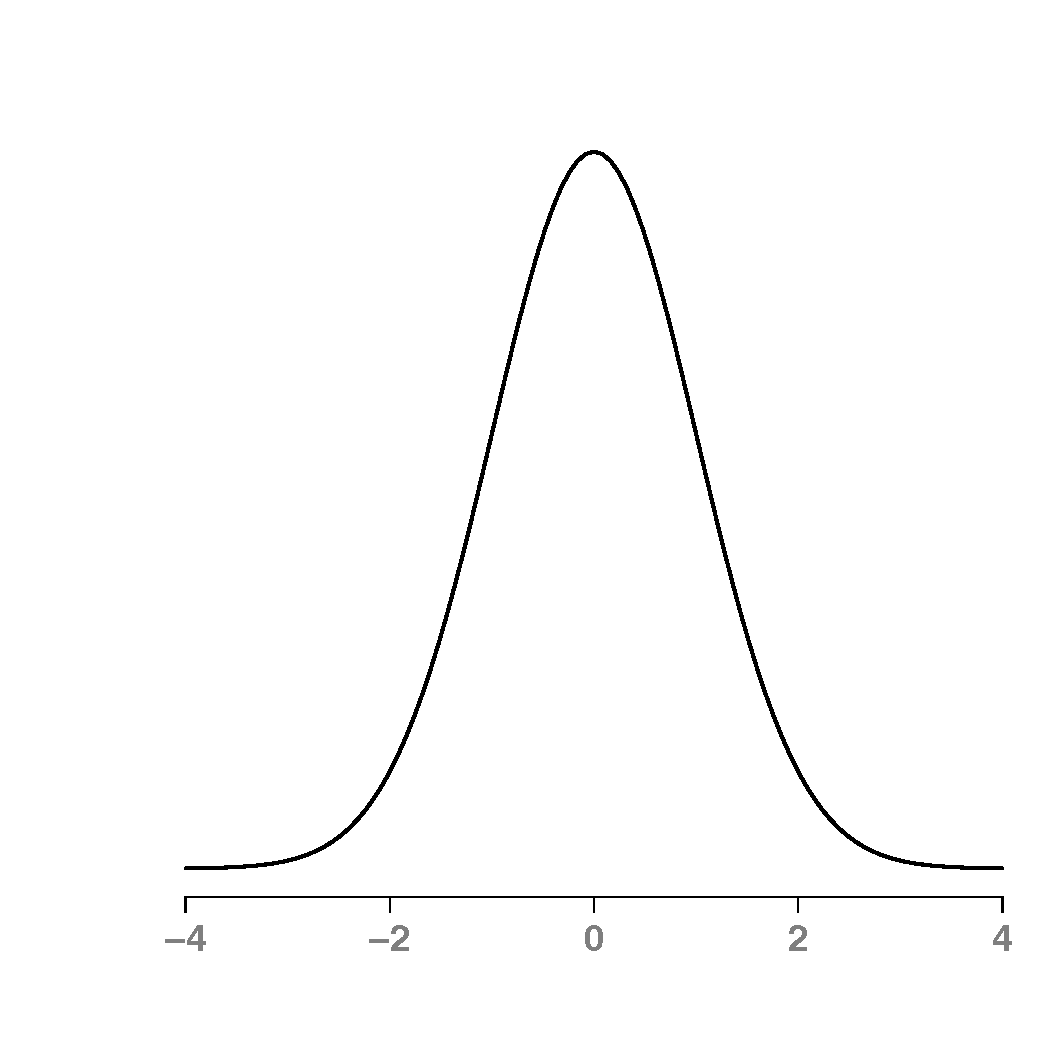
\includegraphics[height=.5\textheight, width = .5\textwidth]{figures/normal.pdf}
\end{flushright}
\end{frame}

\begin{frame}[t]
  \note[item]{Here's an exercise to build more intuition.}
  \begin{exampleblock}{From the Journal of Empirical Fashion}
  \begin{tabular}{c | c | c}
  & New Yorkers & San Franciscans \\
  \hline
black outfits &  12.1 & 13.3  \\
sample size & 50 & 50
 \end{tabular}
 \end{exampleblock}
   Let $X_1,...,X_{50}$ rep. New Yorkers. Assume iid, mean $\mu_X$.\\
      Let $Y_1,...,Y_{50}$ rep. San Franciscans. Assume iid, mean $\mu_Y$.\\
      Assume $\V[X] = \V[Y] = 4.$
 \note[item]{$z = \frac{\bar{X} - \bar{Y}}{\sigma \sqrt{\frac{1}{n_1}+\frac{1}{n_2}}} = \frac{12.1 - 13.3}{2 \sqrt{\frac{1}{50}+\frac{1}{50}}} = \frac{-1.2}{2 \sqrt{\frac{1}{25}}}  = -3.0$}
 \note[item]{$z>1.96$ REJECT}
 \note[item]{We can also compute p-value 2*pnorm(-3) = .0027}
 \end{frame}



\begin{frame}
  \frametitle{General Procedure for Testing}
  \note[item]{From this example, I hope you see that the two-sample t-test is not all that different from the one-sample tests we did earlier.}
  \note[item]{No matter what the test is, there's a general pattern that you follow...}
  
  Three steps:
  \begin{enumerate}
      \item Specify model and null hypothesis
      \item Calculate $z$ or $t$ statistic
      \item Plot statistic on the null distribution to get the $p$ value.
  \end{enumerate}
\end{frame}


%Section 7.08 New section on t-tests

\section{The Two-Sample t-Test}


\begin{frame}
  \frametitle{Types of Two-Sample t-Tests}
  \note[item]{There are actually two versions of the two-sample t test you should be aware of.}
\note[item]{Student's t-test is the original t-test. it's simpler, but requires strong assumptions}
\note[item]{Welch's t-test is more general, and this is really the modern t-test.}
  \begin{enumerate}
  \item Student's t-Test
  \item Welch's t-Test
 \end{enumerate}
\end{frame}


\begin{frame}
  \frametitle{Student's t-Test}

  $$t = \frac{\mu_{1}-\mu_{2}}{S_{\mu_{1}-\mu_{2}}} $$

  $$
    S_{\mu_{1}-\mu_{2}} = \sqrt{ \left(\frac{ (N_{1}-1)S_{1}^{2} + (N_{2}-1)S_{2}^{2} }{ N_{1}+N_{2}-2 }\right)
                    \left(\frac{1}{ N_{1} } + \frac{1}{ N_{2} }\right)
                  }
  $$

  $$
    t = \frac{(mean\ of\ group\ 1) - (mean\ of\ group\ 2)}{standard\ error\ of\ difference\ between\ means}
  $$
  
  
  \begin{exampleblock}{\textit{t} value}
    \textbf{Difference between group means} (mean difference), divided by the \textbf{variability of the two groups} (standard error of the differences)
  \end{exampleblock}

\end{frame}


\begin{frame}
  \frametitle{Degrees of Freedom}
  
  \begin{exampleblock}{degrees of freedom \textit{(df)}}
    Number of independent pieces of information that vary given model parameters
  \end{exampleblock}
  
  \begin{itemize}
      \item \textbf{One sample t-test}
    \begin{itemize}
      \item \textit{df} = $n - 1$ (only uses one known quantity)
      \item Tests whether one sample's mean is significantly different from some hypothesized mean
    \end{itemize}
    \item \textbf{Student's two-sample t-test}
    \begin{itemize}
      \item Uses two known quantities (the two group means)
      \item \textit{df} = $n_{1} + n_{2} -2$
    \end{itemize}

  \end{itemize}

\end{frame}

\begin{frame}
  \frametitle{Welch's t-Test}
\end{frame}

%Section 7.08 Edits end




\section{Practical Significance of the T-Test}
\begin{frame}
  \frametitle{Practical Significance for the T-Test}

  After using a t-test to assess statistical significance, it is
  important to assess practical significance. \\ \vspace{1em}

  \begin{quote}
    Your main goal is to explain to your audience
    why they should or should not care about the effect.
  \end{quote}

  \textbf{Three common effect size measures:}

  \begin{enumerate}
  \item Difference in means
  \item Cohen's d
  \item Correlation r
  \end{enumerate}
\end{frame}

\begin{frame}
  \frametitle{Difference in Means}

  \begin{block}{Difference in means}
    \[
      \overline{X}_{A} - \overline{X}_{B}
    \]
  \end{block}
    \begin{itemize}
    \item Answers the question ``\textit{How different are these
        groups?''}
    \item Often makes great headlines
      and is a good choice if units are familiar
    \item But lacks context in its calculation
  \item People who eat chocolate live 1.5 years longer than those who
    do not each chocolate
  \end{itemize}
\end{frame}


  \begin{frame}
    \frametitle{Cohen's d}

    \begin{block}{Cohen's d}
      \small
    \textit{Cohen's d} is a measure of difference of means
    standardized by the variance in the data.
    \[
      \frac{ \overline{X}_{A} - \overline{X}_{B} }{s}
    \]
    Where $s$ is a pooled standard deviation:
    $\sqrt \frac{(n_1-1)s_1^2 + (n_2-1)s_2^2}{n_1+n_2}$
  \end{block}

  \begin{itemize}
  \item Answers the question ``\textit{How many standard
      deviations apart are the groups?}''
  \item The difference in sarcasm score between frequentists and
    Bayesians is $d = 0.54$ standard deviations.
  \end{itemize}
\end{frame}

\begin{frame}
  \frametitle{Correlation}
  \note[item]{Notice the similarity in the form between Cohen's d and
    correlation -- Cohen's d divides by the pooled standard deviation;
    correlation divides by the product of two group standard
    deviations.}
  \begin{block}{Correlation}
    \textit{Correlation} answers the question ``How strong is the
    relationship between group identity and the outcome?''
    \[
      \rho = \frac{\cov(X, Y)}{\sigma_{X}\sigma_{Y}}
    \]
  \end{block}

  \begin{center}
    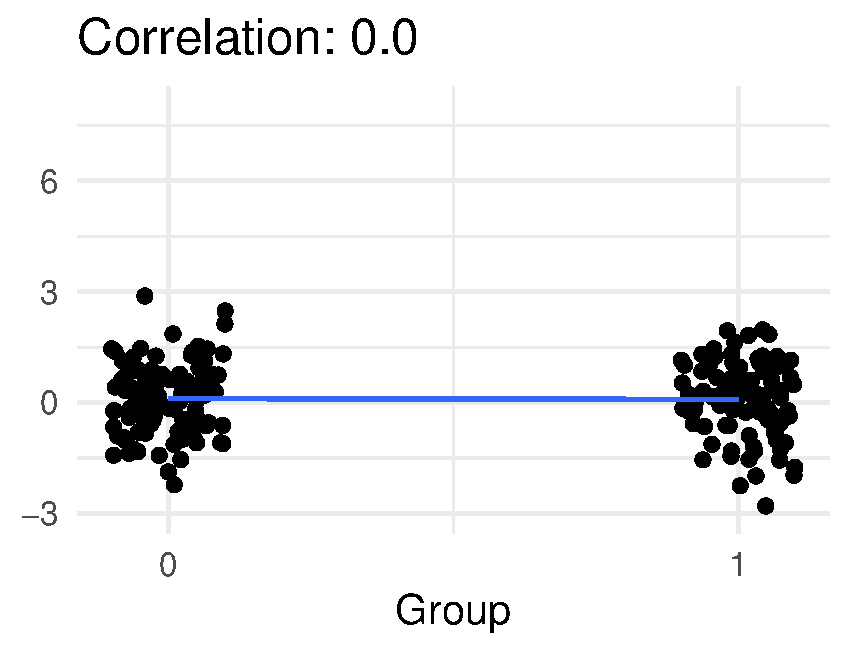
\includegraphics[width = 0.5\linewidth]{./figures/biserial_00}
  \end{center}
\end{frame}

\begin{frame}
  \frametitle{Correlation}

  \begin{block}{Biserial correlation}
    \textit{Correlation} answers the question ``How strong
    is the relationship between group identity and the outcome?''
    \[
      \rho = \frac{\cov(X, Y)}{\sigma_{X}\sigma_{Y}}
    \]
  \end{block}

  \begin{center}
    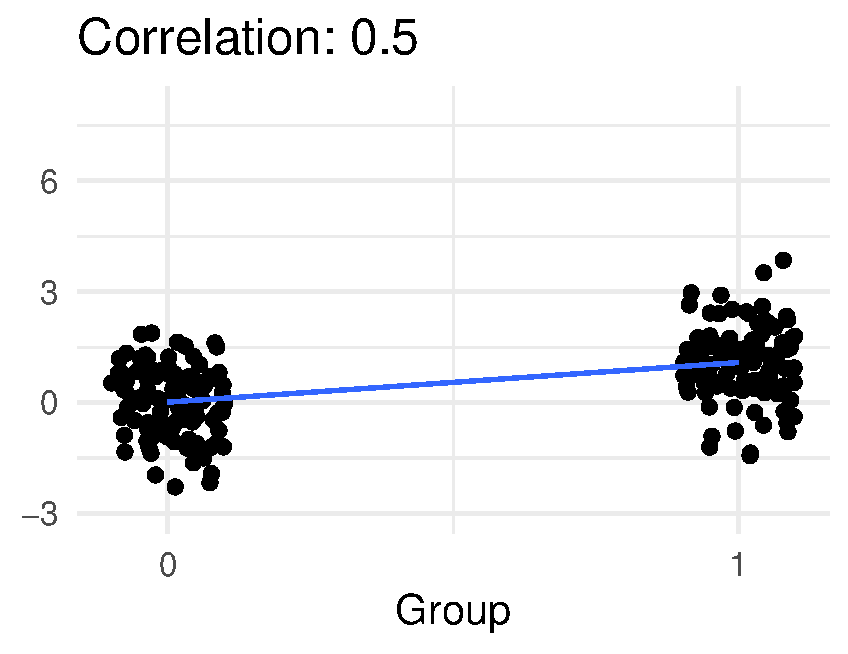
\includegraphics[width = 0.4\linewidth]{./figures/biserial_05}
  \end{center}
\end{frame}

\begin{frame}
  \frametitle{Correlation}

  \begin{block}{Biserial correlation}
    \textit{Correlation} answers the question ``How strong
    is the relationship between group identity and the outcome?''
    \[
      \rho = \frac{\cov(X, Y)}{\sigma_{X}\sigma_{Y}}
    \]
  \end{block}

  \begin{center}
    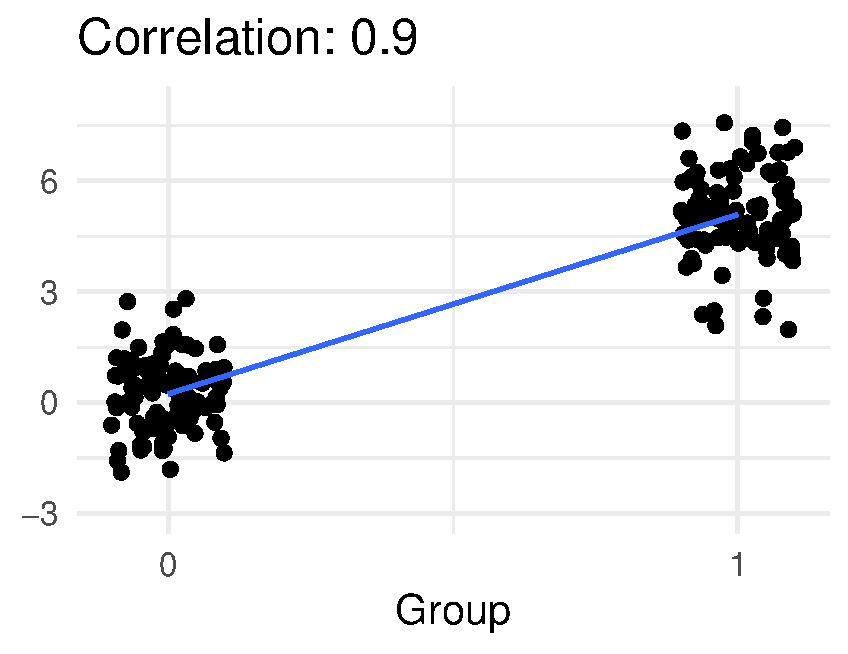
\includegraphics[width = 0.4\linewidth]{./figures/biserial_09}
  \end{center}
\end{frame}

\begin{frame}
  \frametitle{Practical Significance is about Context}

  \begin{itemize}
  \item How strong is the same relationship between \textit{different}
    groups?
  \item How strong is a \textit{different} relationship between the
    same group?
  \item What is the underlying dispersion in the data?
  \item What is a meaningful anchor or reference point that you can
    use for context?
  \end{itemize}
\end{frame}

\section{The Paired t-Test}

\begin{frame}
  \frametitle{Paired t-Test}

  \begin{exampleblock}{Climbing grip}
    Suppose you randomly sample 30 Berkeley students.  For each
    student $i$, you measure right-hand strength ($R_i$) and left-hand
    strength ($L_i$).

    \begin{itemize}
    \item You conduct a t-test with $H_0: \E[R] = \E[L]$
    \item \textbf{Problem}: Grip strength varies a lot
      person-to-person, $\Rightarrow$  t-test has low power.
    \end{itemize}
  \end{exampleblock}
\end{frame}

\begin{frame}
  \frametitle{Paired t-test}
  \centering
  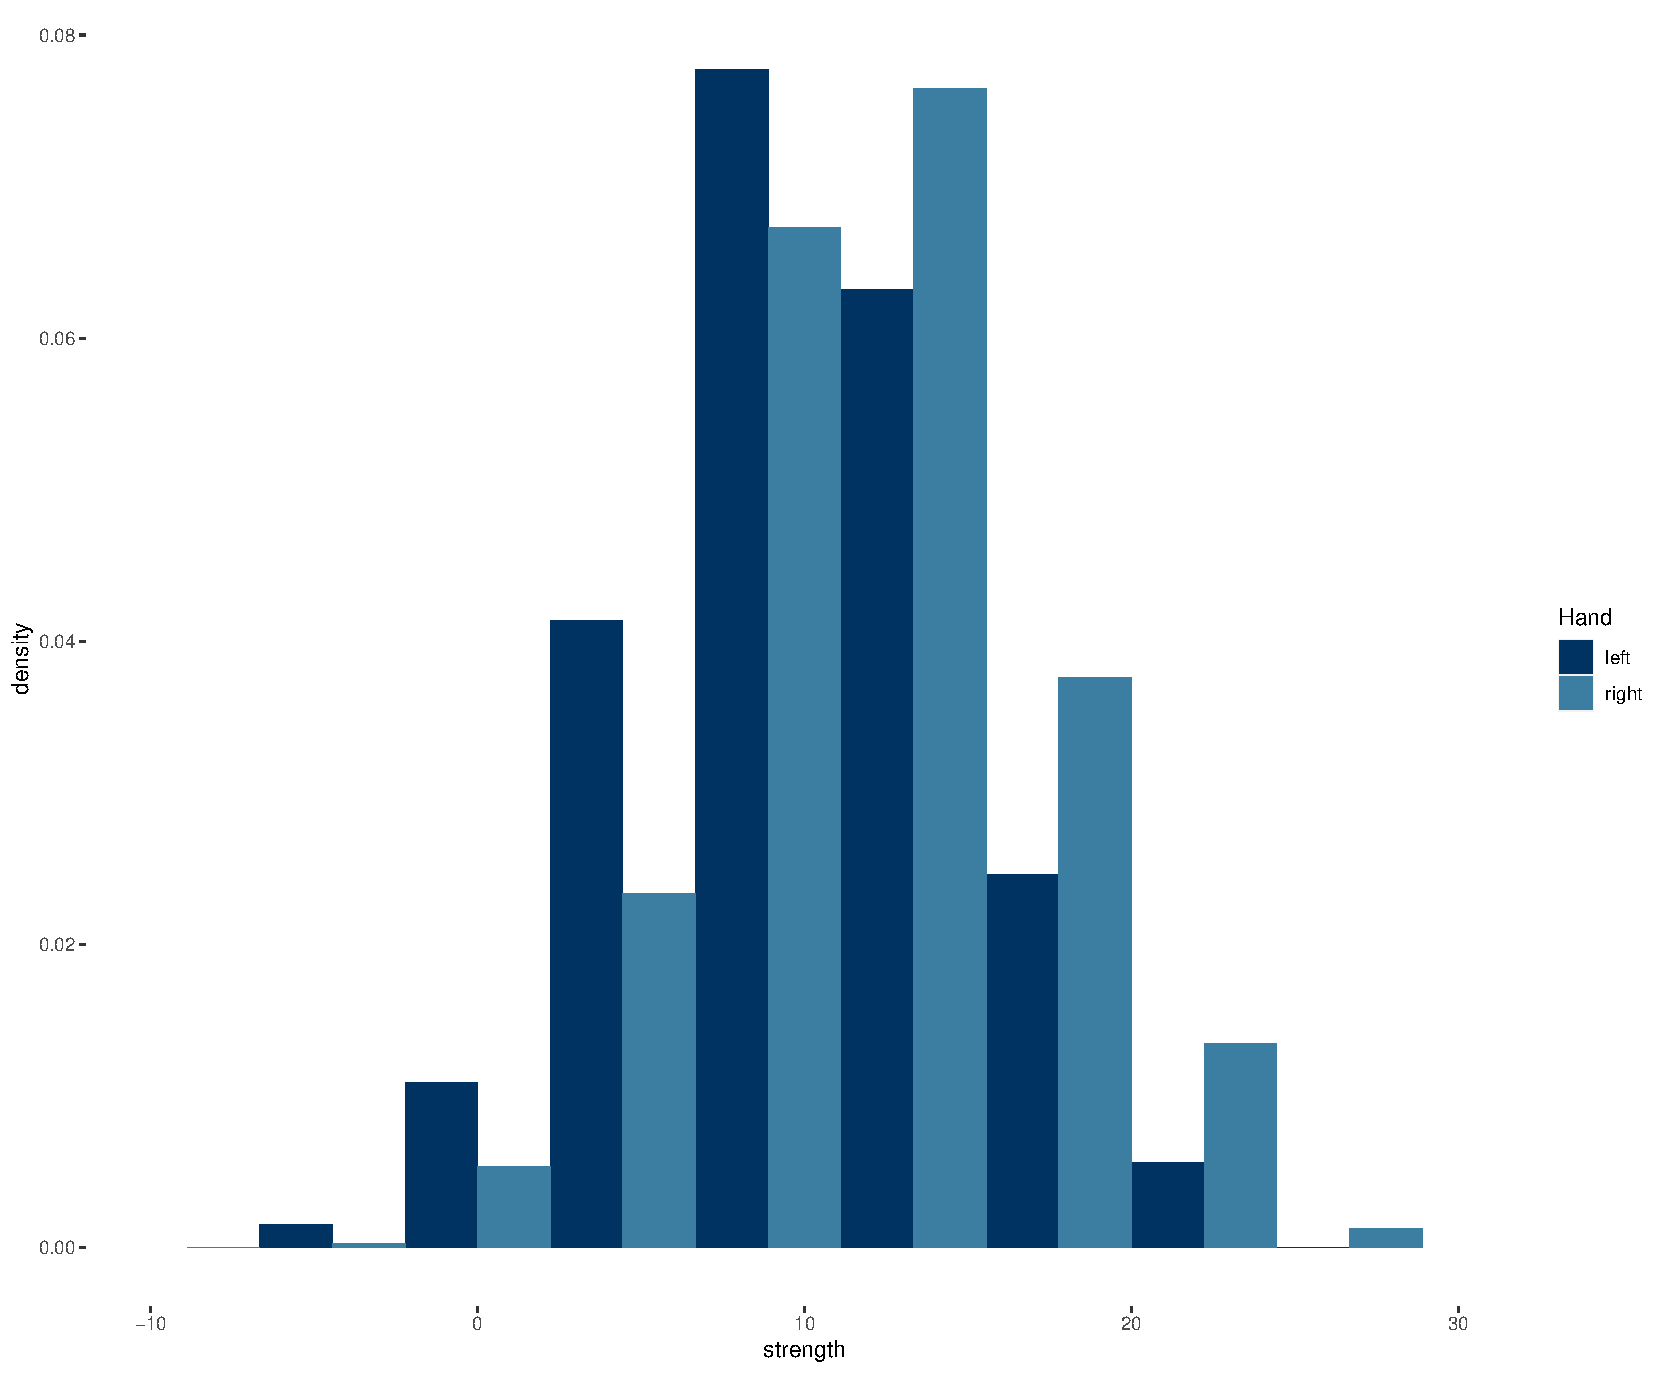
\includegraphics[width=.9\linewidth]{./figures/histogram_unpaired.pdf}
\end{frame}

\begin{frame}
  \frametitle{Paired t-Test}

  \begin{itemize}
  \item \textbf{Idea:} For any \textit{particular} subject $i$, the difference
    between right-hand strength and left-hand stregth, $R_i - L_i$,
    will usually be small.
  \item Within-person variation is small.
  \end{itemize}

  \begin{center}
    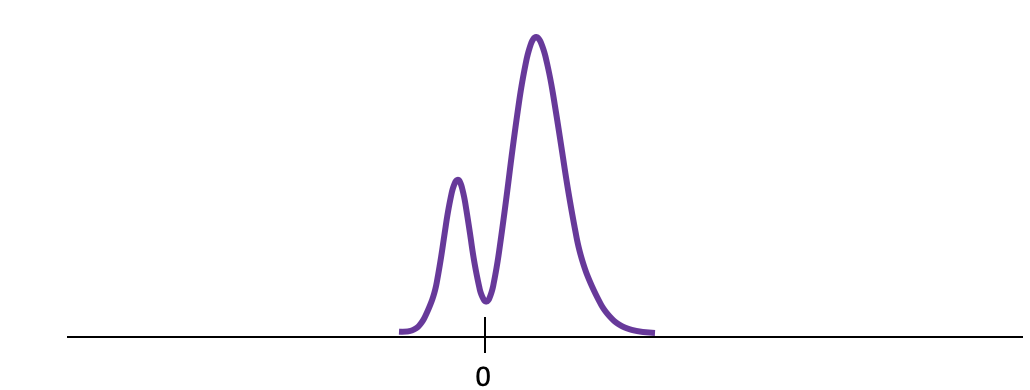
\includegraphics[width=.9\linewidth]{./figures/grip}
  \end{center}
\end{frame}

\begin{frame}
  \frametitle{Paired t-Test}
  \centering
    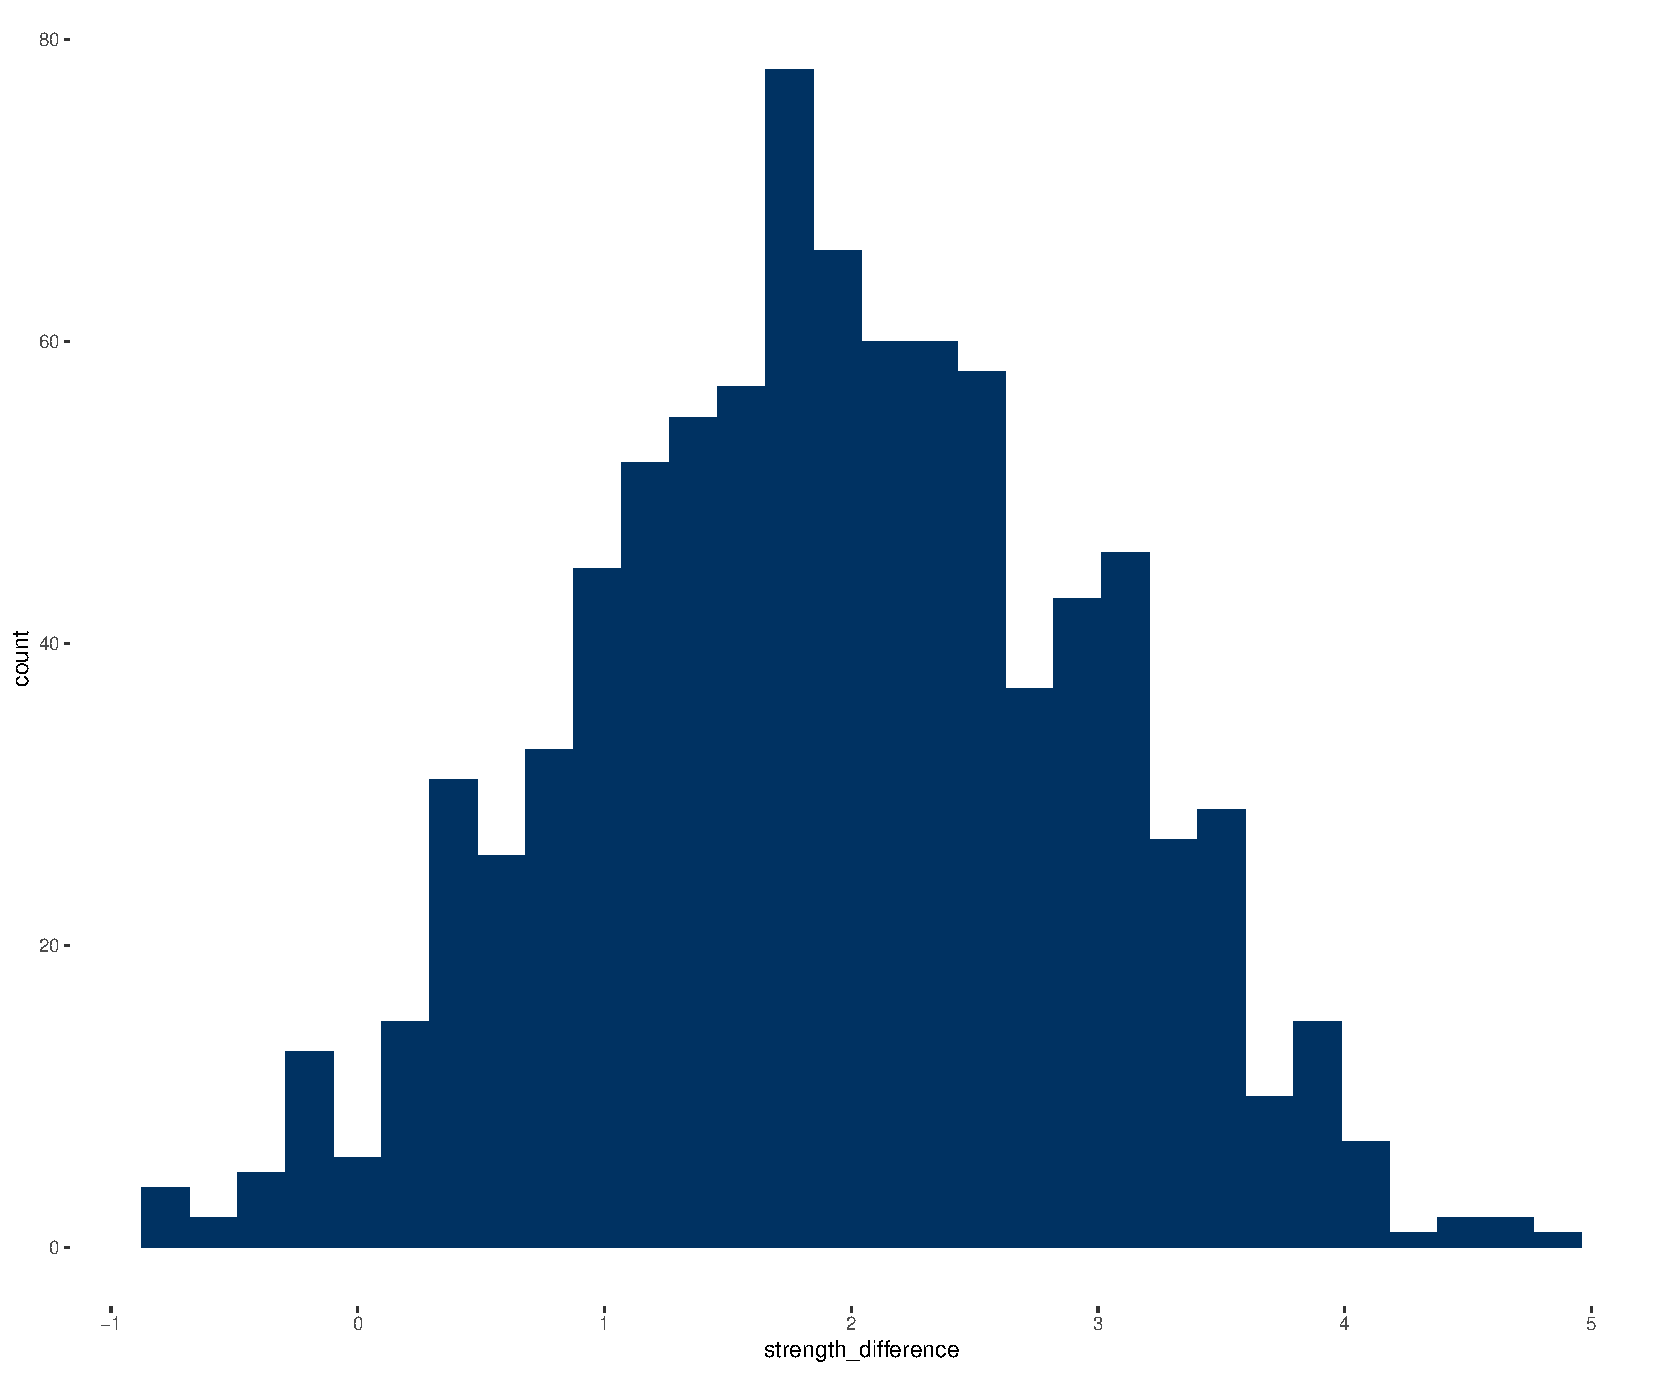
\includegraphics[width=.9\linewidth]{./figures/histogram_paired.pdf}
\end{frame}

\begin{frame}
  \frametitle{Paired t-Test}
  \centering
    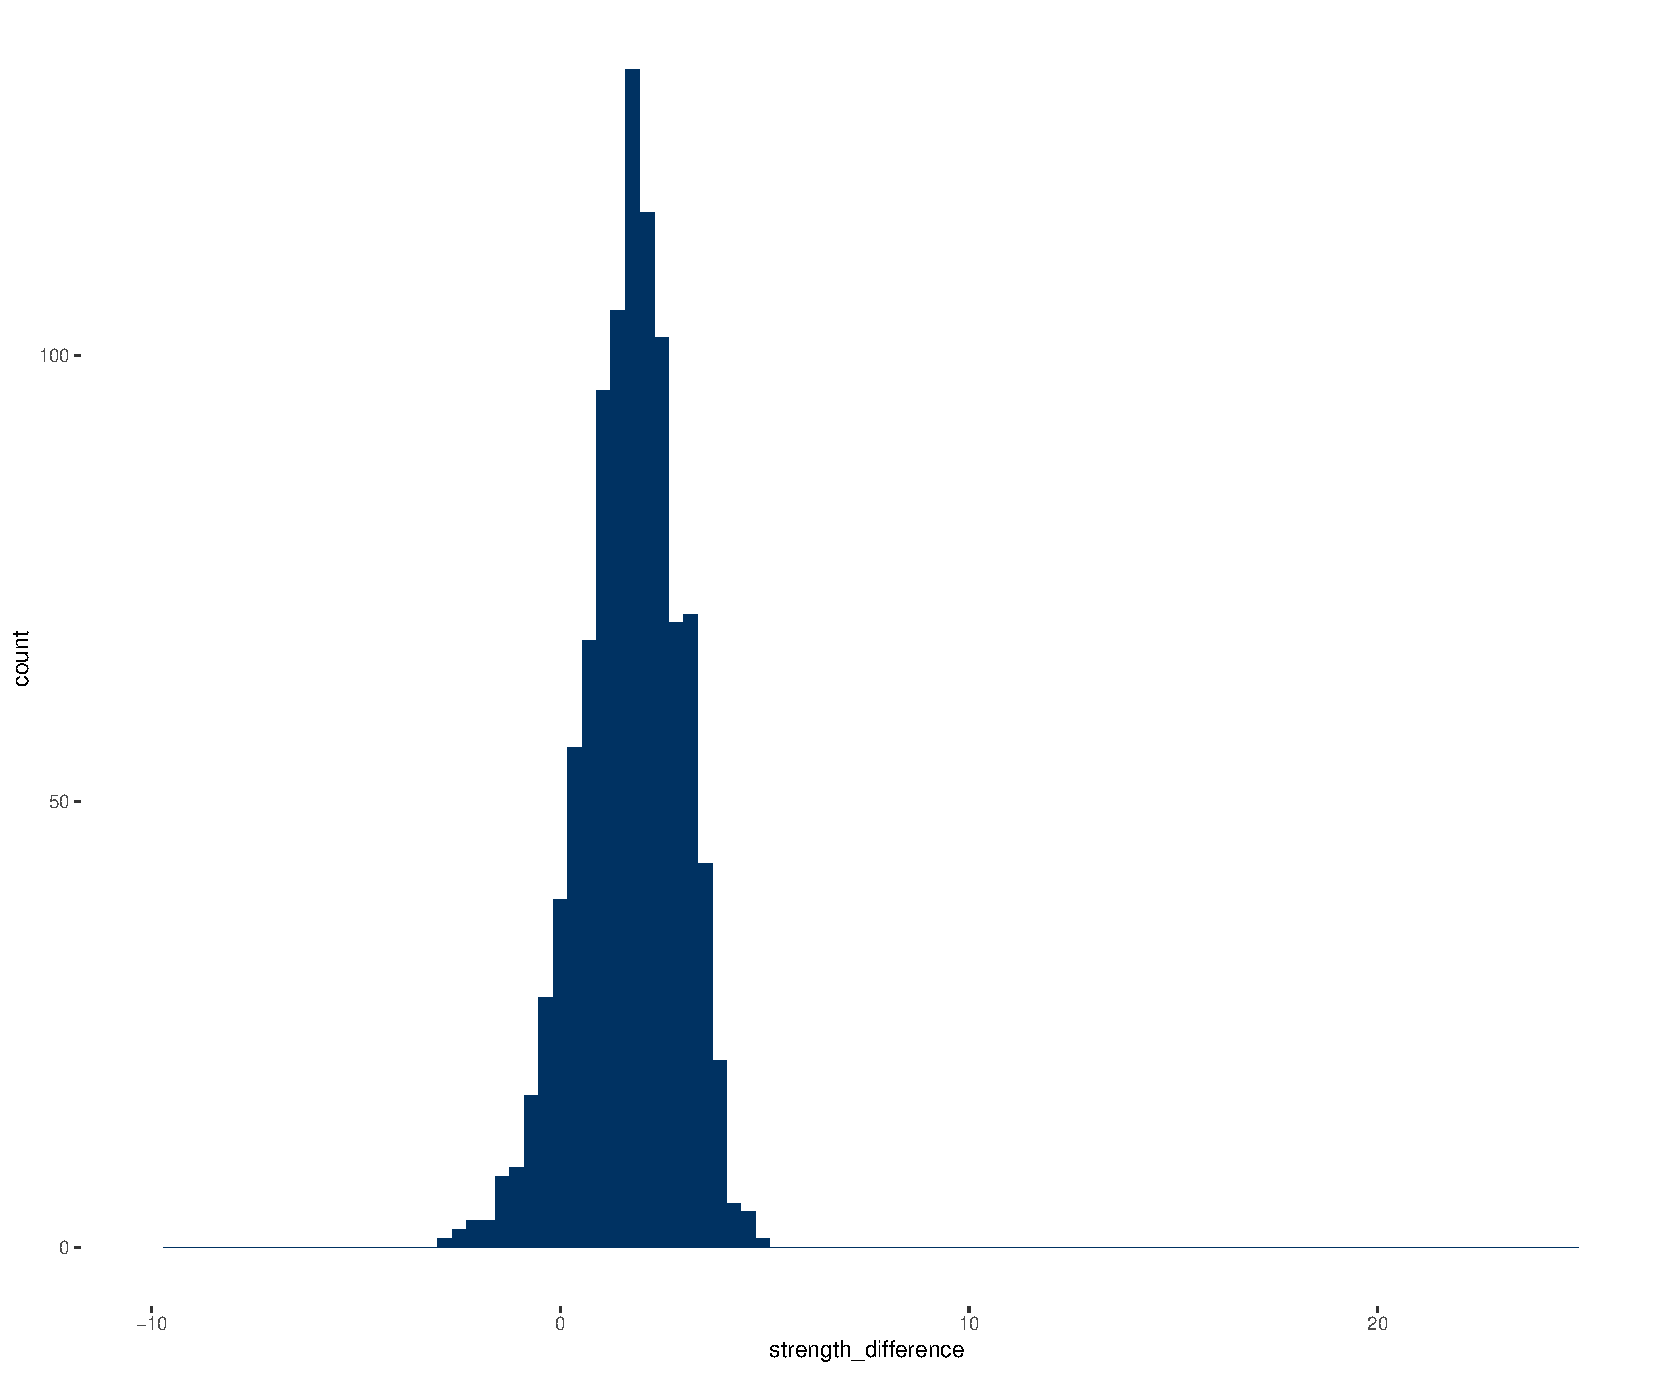
\includegraphics[width=.9\linewidth]{./figures/histogram_paired_rescaled.pdf}
\end{frame}

\begin{frame}
  \frametitle{Paired t-Test}
  \begin{block}{Paired t-test}
    A \textit{paired t-test}, sometimes called a \textit{dependent
      t-test}, builds an explicit dependency between data.
    Instead, perform a one-sample t-test with $H_0: \E[ R_{i}- L_{i}] = 0$.
  \end{block}
  \begin{itemize}
  \item This dependency must actually exist
  \item Cannot simply change the test
  \end{itemize}
\end{frame}

\begin{frame}
  \frametitle{Unpaired vs. Paired t-Test}

  \begin{columns}[t]
    \column{.49\linewidth}
    \textbf{Unpaired}
    \begin{itemize}
      \item $t = \frac{\overline{A} - \overline{B}} {\sigma_{A\&B}}$
    \end{itemize}
    \column{.49\linewidth}
    \textbf{Paired}
    \begin{itemize}
    \item $t = \frac{\overline{A} - \overline{B}}{\sigma_{(A - B)}}$
    \end{itemize}
  \end{columns}

\end{frame}

\begin{frame}
  \frametitle{Paired t-Test Assumptions}

  \begin{itemize}
  \item $A$ and $B$ have a metric scale with the same units.
  \item There is a natural pairing between observations for $A$ and for $B$.
    \begin{itemize}
    \item pre-test and post-test for same individual
    \item response to two types of stimulus for same mouse
    \item responses for a pair of spouses
    \end{itemize}
  \item Each pair $(A_i, B_i)$ is drawn i.i.d.
  \item The distribution of $A-B$ is sufficiently normal given the sample size.

  \end{itemize}
\end{frame}



%Start section 7.17 edits
\section{Introduction to Non-parametric Tests}

\begin{frame}
  \frametitle{Non-parametric Tests}
  
  \begin{itemize}
    \item $t$-test is parametric, like all the tests we've seen so far
    \begin{itemize}
      \item Assumes the population comes from a parametric family of distributions
      \item Typically the normal curves
    \end{itemize}
    \item It is not always possible to meet this assumption
  \end{itemize}
  
\end{frame}


\begin{frame}
  \frametitle{Non-parametric Tests (cont.)}    

  \textbf{Large sample} 
  \begin{itemize}
    \item No Problem
    \item central limit theorem tells us that the sampling distribution of the mean will be approximately normal, so $t$-tests are valid
    \item Parametric tests are generally valid for large samples
  \end{itemize}

\end{frame}


\begin{frame}
  \frametitle{Non-parametric Tests (cont.)}
  
  \textbf{Small sample}
  \begin{itemize}
    \item $t$-test is fairly robust to deviations from normality, but you should look at your distribution and see how non-normal it is
    \item Suppose you have a small sample and you suspect you have a major deviation from normality
    \item You might be able to transform the variable to make it more normal, but that can alter the meaning and make results harder to interpret
  \end{itemize}
  
  
  \begin{exampleblock}{An alternative is to use a \textit{non-parametric} test}
    
  \end{exampleblock}
  
    
\end{frame}

\begin{frame}
  \frametitle{Non-parametric Test Details}
  
  \begin{itemize}
      \item Non-parametric tests can be also called \textbf{distribution- free tests}
      \begin{itemize}
          \item Still involve assumptions, but they are less restrictive than those of parametric tests
      \end{itemize}
      \item Many tests work on principle of ranking data
      \begin{itemize}
          \item List the scores from lowest to highest -- each score gets a rank, so higher scores have higher ranks
          \item Only consider ranks instead of looking at the metric value of the variable
          \item Use the order of variables to construct statistics that we can use to test hypotheses
      \end{itemize}
  \end{itemize}
    
\end{frame}


\begin{frame}
  \frametitle{Non-parametric Test Details (cont.)}
  \begin{columns}
    \column{0.5\textwidth}
    \textbf{Advantages}
    \begin{itemize}
        \item Population distribution doesn't have to be normal
        \item Easier to justify a rank-based test
    \end{itemize}
    
    \column{0.5\textwidth}
    \textbf{Disadvantages}
    \begin{itemize}
        \item We throw out metric information
        \item Rule of thumb: if you throw away information, you lose statistical pwoer
    \end{itemize}
  \end{columns}
    
\end{frame}


\begin{frame}
  \frametitle{Rank-Based Tests for Ordinal Variables}
  \begin{itemize}
      \item Rank-based tests are especially useful when we have an ordinal variable 
      \begin{itemize}
          \item eg. a Likert variable such as "how do you feel about a presidential campaign?"
          \item Neutral, support, strongly support, etc.
      \end{itemize} 
      \item It is hard to argue that the difference between neutral and support is the same as the difference between support and strongly support
  \end{itemize}
    
\end{frame}


\begin{frame}
  \frametitle{Love Tester Example}
  
  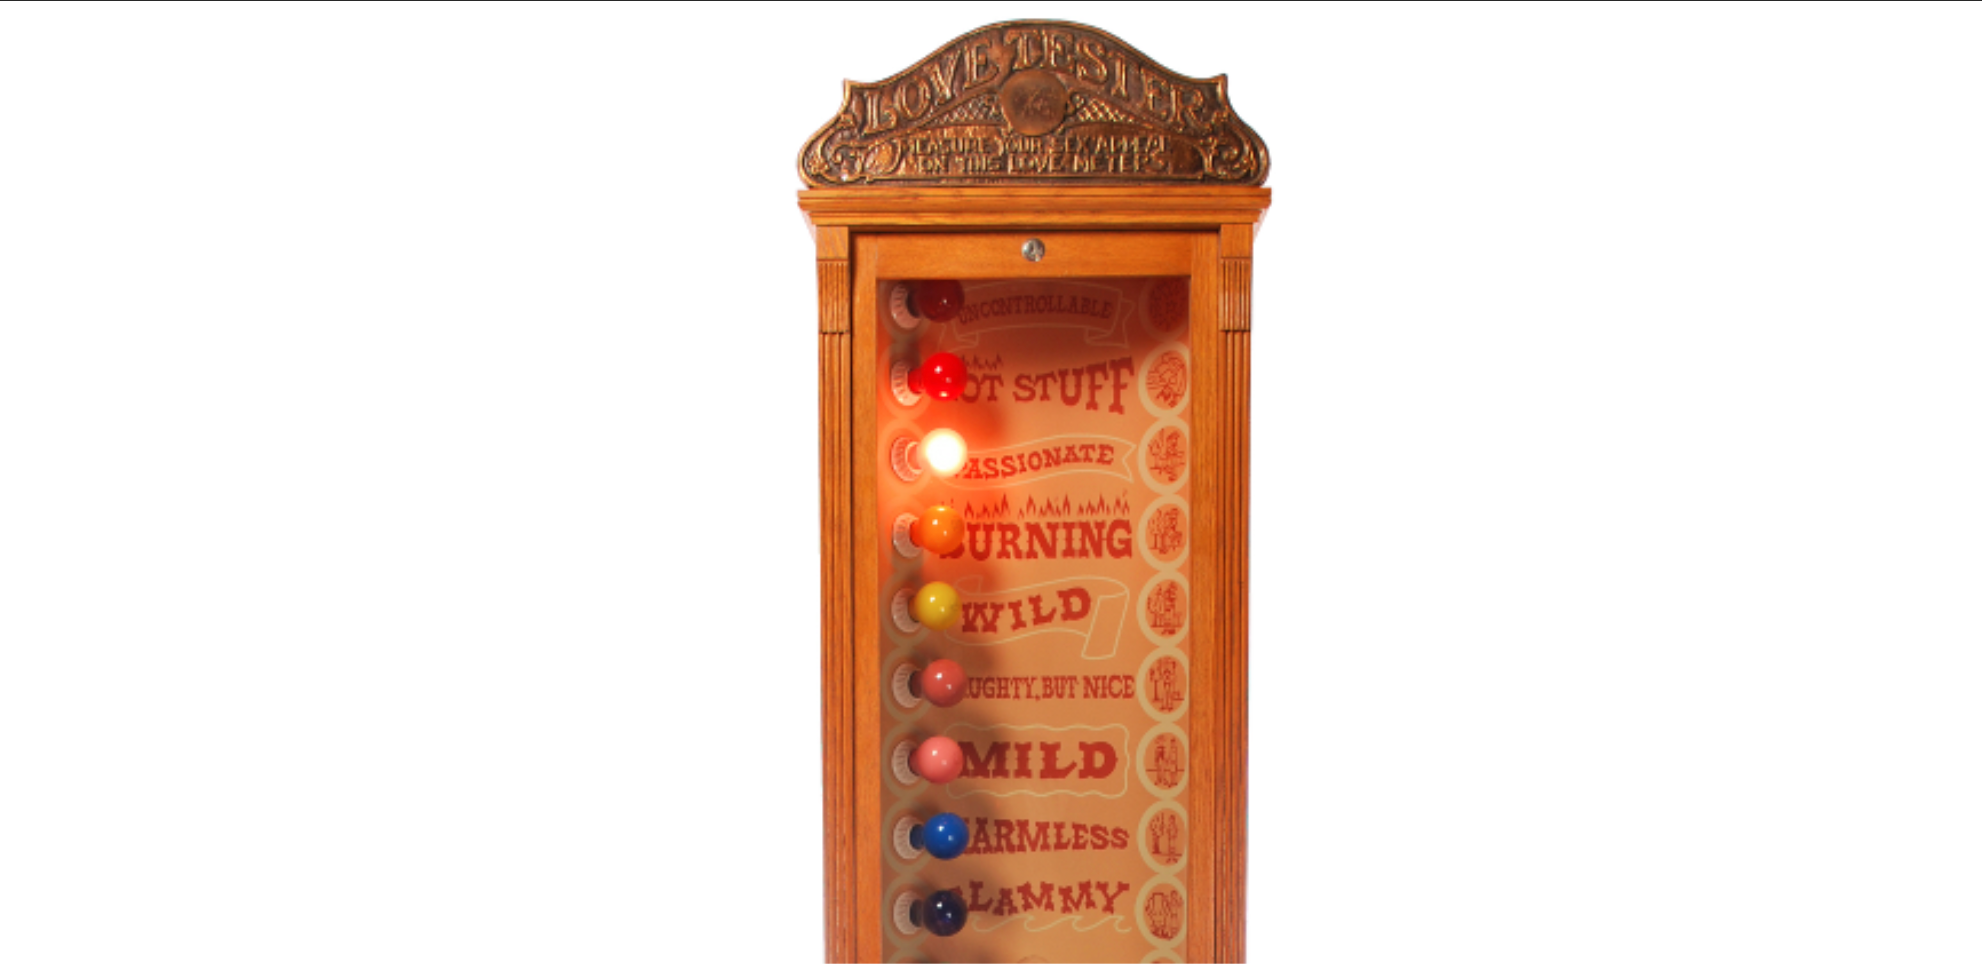
\includegraphics[width=1.0\textwidth]{figures/love_tester.png}

  Do you trust that the difference between harmless and mild is the same as the difference between burning and passionate?
    
\end{frame}

\begin{frame}
  \frametitle{Rank-Based Tests for Ordinal Variables (cont.)}
  
  If you run a $t$-test in these cases, you impose a linear structure on your variable, treating it as metric
  \begin{itemize}
      \item This method may or may not be reasonable
      \item If you use a rank-based test that is okay--you are asking whether one group tends to rank below or above another 
      \item The ranks are still meaningful
  \end{itemize}
    
\end{frame}


\begin{frame}
  \frametitle{Conclusion}

  \begin{itemize}
    \item There are some situations in which you should consider non-parametric tests
    \item Coye is going to tell you more about the specifics
  \end{itemize}
  
\end{frame}




%End section 7.17 edits







%Start section 7.19 edits
\section{Wilcoxon Rank-sum Test for Independent Groups}


\begin{frame}
  \frametitle{Parametric and Non-parametric Tests for Comparing Only Two Groups}

  \begin{center}
    \begin{tabular}{p{0.3\linewidth}||p{0.3\linewidth}|p{0.3\linewidth}}
      \textbf{Type of Design} & \textbf{Parametric Tests} & \textbf{Non-parametric Tests}  \\
      \hline \hline
      \textit{Two independent samples}  & Independent samples $t$ test & Wilcoxon rank-sum test (Mann-Whitney test) \\
      \hline
      \textit{Two dependent Samples } & Dependent samples $t$ test & Wilcoxon signed-rank test
    \end{tabular}   
  \end{center}

\end{frame}


\begin{frame}
  \frametitle{Comparing Two Independent Conditions: Wilcoxon Rank-Sum Test}
  
  \begin{itemize}
    \item Data are ranked from lowest to highest across groups
    \item This provides \textbf{potential rank} scores
    \item If the same score occurs more than once then all scores of the same value receive the average of the potential ranks for those scores
  \end{itemize}
  
  \begin{center}
    \scalebox{0.4}{  
      \begin{tabular}{c|cccc}
        ID & Group & Score & Potential Rank & Final Rank \\ \hline
        1  & A     & 10    & 1              & 1   \\ 
        2  & A     & 11    & 2              & 2.5 \\ 
        3  & B     & 11    & 3              & 2.5 \\ 
        4  & B     & 12    & 4              & 4   \\ 
        5  & A     & 20    & 5              & 6   \\
        6  & B     & 20    & 6              & 6   \\
        7  & B     & 20    & 7              & 6   \\
        8  & A     & 33    & 8              & 8   \\
      \end{tabular}
    }
  \end{center}

  \begin{itemize}
      \item This gives us the \textbf{final rank} scores
  \end{itemize}
\end{frame}


\begin{frame}
  \frametitle{Comparing Two Independent Conditions: Wilcoxon Rank-Sum Test}

  \begin{center}
    \begin{tabular}{c|cccc}
      ID & Group & Score & Potential Rank & Final Rank \\ \hline
      1  & A     & 10    & 1              & 1   \\ 
      2  & A     & 11    & 2              & 2.5 \\ 
      3  & B     & 11    & 3              & 2.5 \\ 
      4  & B     & 12    & 4              & 4   \\ 
      5  & A     & 20    & 5              & 6   \\ 
      6  & B     & 20    & 6              & 6   \\ 
      7  & B     & 20    & 7              & 6   \\ 
      8  & A     & 33    & 8              & 8   \\
    \end{tabular}
  \end{center}

\end{frame}


\begin{frame}
  \frametitle{Calculating the Wilcoxon Rand-Sum Test}
  
  \begin{itemize}
    \item After assigning final ranks, add up all the final ranks for each of the two groups
    \item Subtract the mean rank for a group of the same size as our groups
    \begin{itemize}
      \item Otherwise, larger groups would always have larger values
      \item For example, the mean group for a group of four = 1 + 2 + 3 + 4 = 10
    \end{itemize}
    \item Our final calculation in therefore:
    \begin{itemize}
      \item $W$ = sum of ranks - mean rank
    \end{itemize}
  \end{itemize}
    
\end{frame}


\begin{frame}
  \frametitle{Calculating the Wilcoxon Rank-Sum Test (cont.)}
  
  \begin{center}
    \scalebox{0.75}{  
      \begin{tabular}{c|cccc}
        ID & Group & Score & Potential Rank & Final Rank \\ \hline
        1  & A     & 10    & 1              & 1   \\
        2  & A     & 11    & 2              & 2.5 \\ 
        3  & B     & 11    & 3              & 2.5 \\ 
        4  & B     & 12    & 4              & 4   \\ 
        5  & A     & 20    & 5              & 6   \\
        6  & B     & 20    & 6              & 6   \\
        7  & B     & 20    & 7              & 6   \\
        8  & A     & 33    & 8              & 8   \\
      \end{tabular}
    }
  \end{center}

  \begin{itemize}
    \item Group A: W = sum of ranks (17.5) - mean rank (10) = 7.5
  \end{itemize}
    
\end{frame}


\begin{frame}
  \frametitle{Interpretation of the Wilcoxon Rank-Sum Test}

  \begin{exampleblock}{Default is a two-sided test, like a \textit{t} test}
    \textbf{Null hypothesis:} There is no difference in ranks
    \textbf{Alternative hypothesis:} There is a difference in ranks
  \end{exampleblock}
  
  \begin{itemize}
      \item You can also do a one-directional test if you hypothesize that one particular group will have higher ranks than the other
      \item Always two values for $W$ (one for each group)
      \item Lowest score for $W$ is typically used as the test statistic
  \end{itemize}
  
\end{frame}

\begin{frame}
  \frametitle{Interpretation of the Wilcoxon Rank-Sum Test (cont.)}
  
  \begin{itemize}
      \item For small sample sizes ($N<40$), R calculates the $p$ value with the Monte Carlo methods
      \begin{itemize}
          \item ie. simulated data are used to estimate the statistic
      \end{itemize}
      \item For larger samples, R calculates the $p$ value with a normal approximation method
      \begin{itemize}
          \item Assumes that the sampling distribution of the $W$ statistic is normal, not the data
          \item Normal approximation method helpful because it calculates a z statistic in the process of calculating the $p$ value
      \end{itemize}
  \end{itemize}
    
\end{frame}

\begin{frame}
  \frametitle{Effect Size for the Wilcoxon Rank-Sum Test}

  \begin{exampleblock}{Effect Size Correlation}
    $$r = \frac{Z}{ \sqrt{N} }$$
    Divide the z statistic by the square root of the total sample size
  \end{exampleblock}

  \begin{center}
  \begin{tabular}{c|c}
    r    & Effect Size  \\ \hline
    0.10 & Small \\
    0.30 & Medium \\
    0.50 & Large 
  \end{tabular}
  \end{center} 
\end{frame}

%End section 7.19 edits

\end{document}
